
\documentclass{acm_proc_article-me}

\usepackage[none]{hyphenat}
\sloppy

\begin{document}
\conferenceinfo{\textit{MediaEval 2014 Workshop,}}{October 16-17, 2014, Barcelona, Spain}

\title{Re-Ranking the Image Search Results for Relevance and Diversity in MediaEval 2014 Challenge}

\numberofauthors{3}

\author{
\alignauthor
Zsombor Par\'oczi\\
       \affaddr{Inter-University Centre for Telecommunications and Informatics}\\
       \email{paroczi@tmit.bme.hu}
\alignauthor
B\'alint Fodor\\
       \affaddr{Inter-University Centre for Telecommunications and Informatics}\\
       \email{balint.fodor@aut.bme.hu}
\alignauthor
G\'abor Sz\H ucs \\
       \affaddr{Inter-University Centre for Telecommunications and Informatics}\\
       \email{szucs@tmit.bme.hu}
}

\maketitle
\begin{abstract}

In this paper we introduce a refinement and diversification process for re-ranking image search results based on social metadata and visual characteristics of the photos.
The goal of the developed re-ranking algorithm is to construct a new sequence with maximal
value of the harmonic mean of precision and diversity. Our contribution is twofold: estimation of precision using the statistical average and mixing of clustering results in order to get better diversity. In the combined clustering the new label set is the Cartesian product of the two original cluster label sets.

\end{abstract}

\section{Introduction}

Many potential tourists do websearches when they try to find more information about a place they are potentially visiting. These people have only a vague idea about the location, knowing the name of the place. Our aim is to help them by providing a set of photos, as summary of the different views of the location. 
In the official challenge of the MediaEval 2014 Retrieving Diverse Social Images task \cite{ionescu2014retrieving} a ranked list of location photos retrieved from Flickr (using text information) is given, and the task is, to refine the results by providing a set of images that are both relevant and provide a diversified summary. The diversity means that images can illustrate different views of the location at different times of the day/year and under different weather conditions, creative views, etc. The refinement and diversification process can be based on the social metadata associated with the collected photos in the data set~\cite{ionescu2014div400} and/or on the visual characteristics of the images. The initial results are typically noisy and redundant because of the imperfect metadata and the current, restricted search capabilities of the social media platforms~\cite{radu2014hybrid}, where the large variety comes from very different users. 

The goodness of the refinement process can be measured using the precision and diversity metric.
%~\cite{Taneva:2010:GRP:1718487.1718541}
In a previous participation in the task we have solved a very similar problem via diversification of initial results using clustering~\cite{szHucs2013bmemtm}, but our solution was focused on diversification only. In this paper we focused on relevance and diversity with the same importance, as a new idea.

\pagebreak
\section{Re-ranking System}

We took five approaches to generate the final re-ranking of the inital search result. This required five different systems that share similar components. The components can be seen in Figure \ref{fig:block}, where the 'relevance scoring' part creates a model, based on this model the 'estimation' component estimates the relevance of test data (optionally using the credibility set), 'clustering' part generates clusters, and 're-ranking' component produces final ranks.

\begin{figure}[t]
\centering
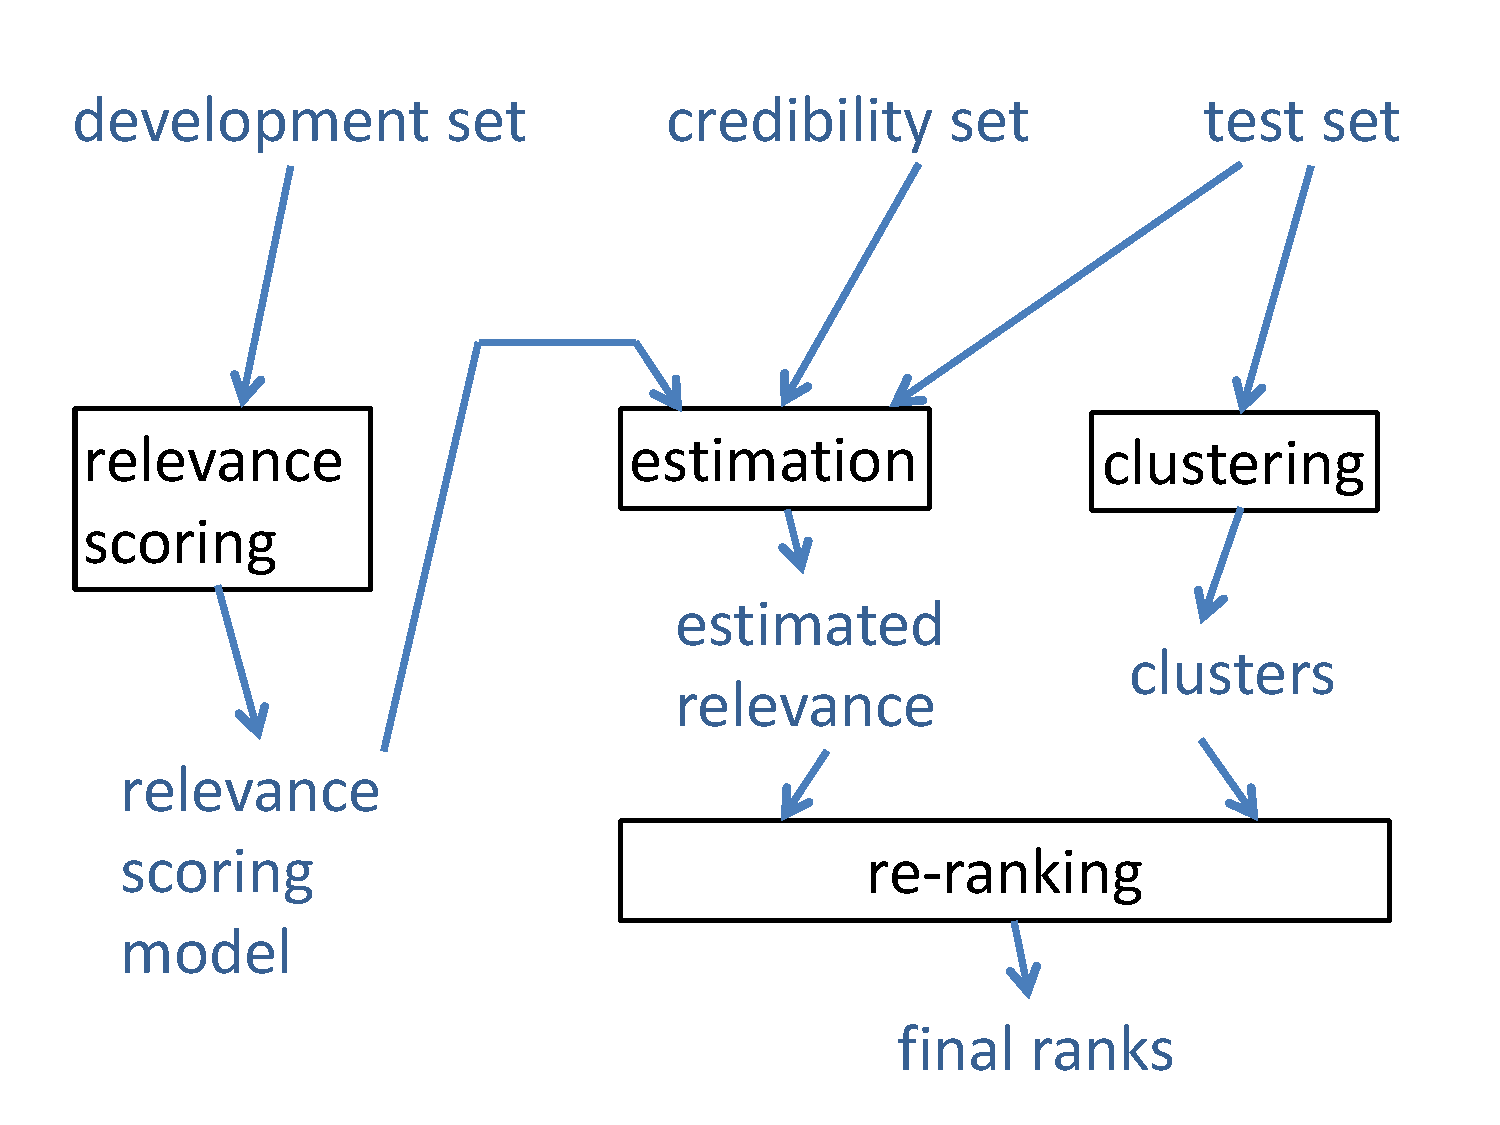
\includegraphics[width=0.8\linewidth]{BlockDiagram}
\caption{System overview}
\label{fig:block}
\end{figure}

All the systems take the inital ranks as input along with the visual feature descriptors and the textual descriptors corresponding to the images. In each case the relevance of all images are estimated, the images are grouped into clusters and based on this two type of information the final ranks are determined.

Section \ref{sec:relevance}. describes the 'average' relevance estimation and its extended versions using user tagging credibility information. Tagging credibilities are used with different weights in the last two approaches. Section \ref{sec:clust}. defines the methods we used to cluster the data.

\subsection{Relevance Scoring and Estimation}
\label{sec:relevance}

For every $k$th place in the initial sequence of the development data set we compute the probability of the item at the $k$th place of being relevant. Before giving the formal definition let denote the set of all initial sequences in the development set as $L$, the $k$th element of the sequence $l \in L$ as $l_k$ and the binary function of the relevance (based on the ground truth data) as $r_{gt}(l_k)$. Then $p_k$, the estimated probability of the $k$th element in an ordering is relevant:
$p_k = \frac{1}{|L|}\sum_{l \in L}r_{gt}(l_k)$.

When processing an initial sequence (from the test data set) we give the relevance score of $p_k$ to the $k$th element of the sequence. In Table \ref{table:runs} 'avg + credibility' means that the relevance estimation is multiplied by the user tagging credibility.

\subsection{Clustering}
\label{sec:clust}

The provided data sets contain visual feature descriptors (color moments, histogram of oriented gradients, etc) in csv files. First, we merged the descriptors into a long feature vector, one vector for each image. Then the components of the vectors are normalized to bring all the data to the same scale. The vectors are clustered with the K-means algorithm by trying all clustering number parameters from 6 to 18. For every clustering the silhouette score~\cite{rousseeuw1987silhouettes} is calculated and the best instance is selected.

Clusterings based on textual and visual data can differ, but merging the two results can be beneficial. Having two clustering functions $c_1(x)$ and $c_2(x)$ that are mapping an image ID to a cluster label, one can construct $c_3(x) = (c_1(x), c_2(x))$ that maps an image ID to a new cluster labeled by the pair of the two original cluster labels. Note that the new label set is the Cartesian product of the two original cluster label sets.

\subsection{Final Re-ranking}

Our re-ranking algorithm (in order to get maximal $F_1$ value in each subset of the answer list) consists of four phases:
%\begin{enumerate}
1) Take the elements in each cluster in descending order and select the element that possessing the largest probability of relevance, this will be the 1st in the reordered list.
2) $L$th step: take the first elements in each cluster as candidate and calculate the estimated $F_1$ measure: \begin{equation} F_1(@L) = \frac{2 \cdot P(@L) \cdot CR(@L)}{P(@L) + CR(@L)} \end{equation}
3) Select the element that has the largest estimated $F_1$ measure and move to the re-ranked list.
4) Continue with phase 2 until we have cluster elements left.
%\end{enumerate}

\section{Results}

\begin{table}[t]
\centering
\caption{Re-ranking approaches.}
\begin{tabular}{|c|c|c|}
	\hline 
	run name & relevance & clustering\tabularnewline
	\hline 
	\hline 
	run1 & avg & visual\tabularnewline
	\hline 
	run2 & avg & textual\tabularnewline
	\hline 
	run3 & avg & visual+textual\tabularnewline
	\hline 
	run4 & avg + credibility 1 & visual+textual\tabularnewline
	\hline 
	run5 & avg + credibility 2 & visual+textual\tabularnewline
	\hline 
\end{tabular}
\label{table:runs}
\end{table}

Table \ref{table:runs} shows the different system compositions we used. 'Avg' is for the 'average' relevance estimation detailed in Section 2.1.
Figure \ref{fig:p} shows the values of $F_1$ for the different runs, while Table \ref{table:results} shows the average P@20, CR@20 and F1@20 results. The results of the five approaches mainly differ in P@N performance. The cluster recall (CR) is almost the same, so P@N has more impact on the $F_1$ score.

%It is interesting that run2 (the approach that uses only textual data for clustering) performs the best in P@20 average and in P@20-50.

The credibility information tends to have negative effect on both P and CR in our tests, compared to the other runs.

However run3 (clustering based on visual+textual data) underperforms run2 in P@20 average, it is more diverse, so the overall F1@20 score is the hightest for run3.

\begin{figure}[t]
\centering
%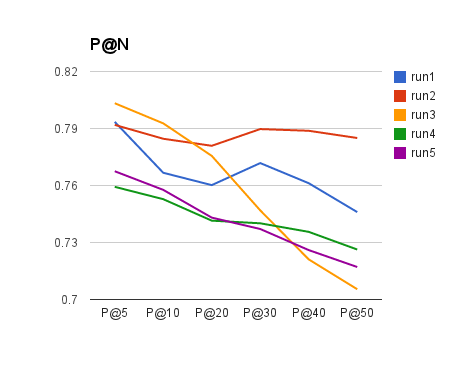
\includegraphics[width=0.8\linewidth]{p}
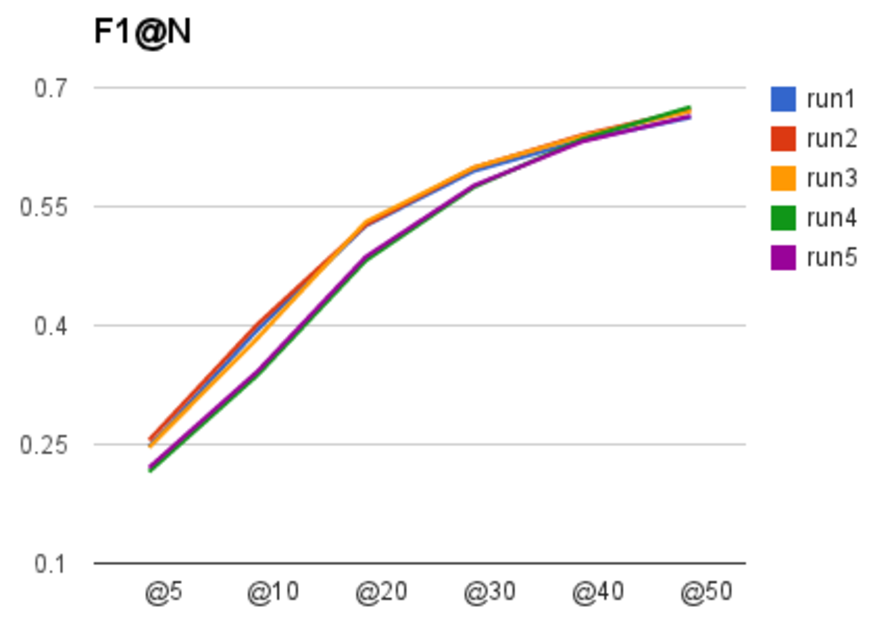
\includegraphics[width=0.95\linewidth]{f1}
\caption{F1@N results}
\label{fig:p}
\end{figure}

\begin{table}[t]
\centering
\caption{Results of the proposed runs on testset}
\begin{tabular}{|l|r|r|r|}
	\hline 
	run name & P@20 & CR@20 & F1@20\tabularnewline
	\hline 
	\hline 
	run1 & 0.7602 & 0.4107 & 0.5259\tabularnewline
	\hline 
	run2 & 0.7809 & 0.4065 & 0.527\tabularnewline
	\hline 
	run3 & 0.7756 & 0.4127 & 0.5305\tabularnewline
	\hline 
	run4 & 0.7415 & 0.3651 & 0.4819\tabularnewline
	\hline 
	run5 & 0.7431 & 0.3682 & 0.4866\tabularnewline
	\hline 
\end{tabular}
\label{table:results}
\end{table}

%\begin{figure}[h]
%\caption{CR@N results}
%\label{fig:cr}
%\end{figure}

%\begin{figure}[h]
%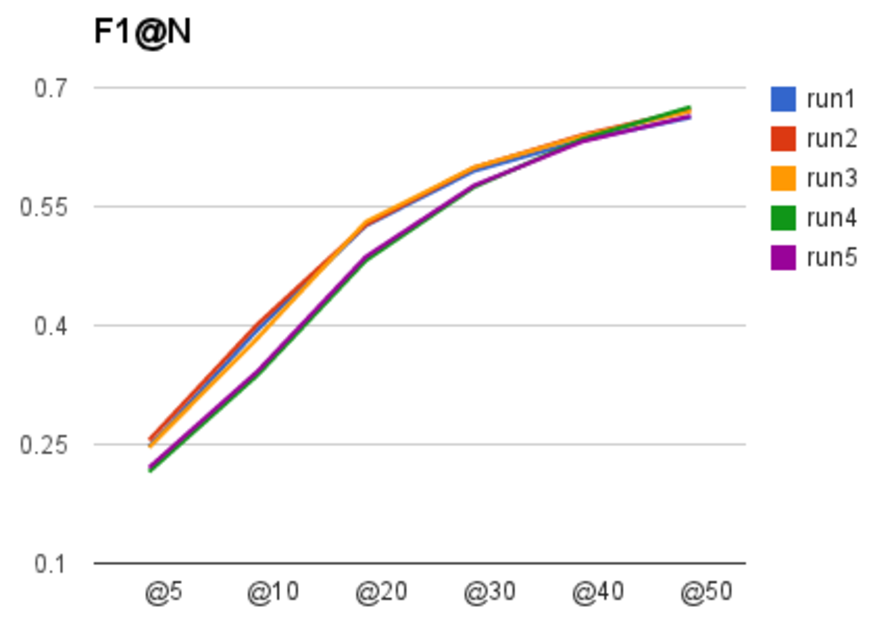
\includegraphics[width=0.9\linewidth]{f1}
%\caption{F1@N results}
%\label{fig:f1}
%\end{figure}

\section{Acknowledgments}

The publication was supported by the T\'AMOP-4.2.2.C-11/1/KONV-2012-0001 project. The project has been supported by the European Union, co-financed by the European Social Fund.

\bibliographystyle{abbrv}
\bibliography{sigproc}

\end{document}
